Speaking about the state of Art, there is a need to explain the current landscape surrounding 4 major 
subjects: \textbf{Blockchain}, \textbf{Hyperledger Fabric},Scalability and 
\textbf{IPFS}. Each one of this topics is important to the given research, since they are considered in at 
least one of the mentioned use cases.

The first one is more about the current general state of the blockchain 
in the healthcare environment,focusing in the overall current play of the blockchain in the world, 
it's influence in healthcare, its benefits, requirements, applications and even the challenges that it is facing.
The second one is more concretely about the \textbf{Hyperledger Fabric} network which is the
framework that is being used in both use cases, having more merit than other private solutions due to its 
time on the market, the enterprise behind it and the number of works that are already published around this 
technology which makes it ideal for this project.The third is Scalability, a crucial huge concern in enterprise 
level contexts because it is the major concept for high availability and meeting the demand of a vast number of 
users. Finally, the forth is about \textbf{IPFS} that plays a role of complementing the blockchain capabilities.

\subsection{Blockchain}
Blockchain technology, introduced in 2008 through the cryptocurrency 
\textbf{Bitcoin}, has been envolving and expanded its influence across numerous sectors within 
\textbf{Information and Communication Technology (ICT)}, with its usage on the rise in recent years. Its adoption 
has been in majority due to the phenomenon of \textbf{cryptocurrencies} \cite{cryptocurrencies-phenomenom} ,
\textbf{CDBS} (Central Bank Digital Currencies) \cite{CDBC} , \textbf{capital investments} and 
\textbf{substantial interesting use cases in blockchain startups} which gathered interest and development of 
this technology. 

This technology operates by storing information in records distributed in a decentralised manner to all computing 
devices within the blockchain infrastructure. The system functions within a peer-to-peer network consisting of 
interconnected nodes. Every node retains its individual copy of the ledger, documenting all transactions within 
the network. The transactions are organised into blocks, each cryptographically linked to the next, forming a 
chain of blocks known as the Blockchain. Thanks to its advanced features, this technology offers multiple services, such as traceability, integrity, and security, while maintaining public and decentralised information storage, thus preserving privacy.
Blockchain technology holds the promise to transform various sectors, including healthcare. Despite the associated
challenges, ongoing research and developments actively address these potential hurdles. As blockchain 
technology progresses, its potential applications and advantages in the
healthcare sector are just beginning to unfold \cite{btc} \cite{healthcare-and-blockchain}. 

\subsection{Types of Blockchain}
Blockchain technology primarily exists in three forms: public (permissionless), 
consortium (public permissioned), and private (permissioned). The main differences between each type of network 
rely on who can access, write, and read data on the Blockchain. In order to come up with a deep understanding over 
it's characteristics, it's worth exploring the specific features of each type \cite{blockchain-in-healthcare}.

Due to their transparency and openness, public blockchains have no barriers to who can use and participate 
in the process, which makes them more decentralized in a certain sense.  The blockchain has publicly visible 
records that anyone on the internet can verify and use to add a transaction block. Examples of public
blockchains include major project networks like \textbf{Bitcoin},\textbf{Ethereum},\textbf{Tron},
\textbf{ICP} and \textbf{solana} where even its use case can be very difference since, as example, 
\textbf{Bitcoin} is meanted to only monetary transactions of information while \textbf{Ethereum}, due to it's 
difference architecture can even run logic over it by leveraging smart 
contracts  \cite{introduction-blockchain} \cite{blockchain-security-issues-and-challenges} \cite{ICP} \cite{solana} \cite{tron-and-eth}.


On the other hand, private blockchains are blockchains in which an organisation 
or entity centralises writing permissions while reading permissions can be public or arbitrarily restricted. 
This means that the configuration of the network is of the responsibility of a single organization. Additionally,
they allow mining and provide high privacy due to writing and reading permissions restrictions. The 
biggest advantage of private blockchains over public ones is that participants can adapt their rules and 
logic according to their business altought a given number of members must agree with each other about this 
rules depending of how the network is configured, allowing them to religiously set what they see as a valid 
transaction within their organization. Moreover, participants and its components are known, restricting any 
addition of forged blocks to the chain. Additionally, altought not recommended manual intervention can correct 
faults and chain participants can control the maximum block size, addressing scalability issues or their proper
use case. Verified participants only verify transactions, leading to lower processing power and cheaper 
transactions. This type of blockchain is similar to a standard distributed database. \textbf{Hyperledger Fabric} 
is the most mentioned permissioned  \cite{data-processing-view-blockchain} \cite{private-blockchain}.

Finally, let's explore the consortium blockchain. This type comprises a set of organisations or entities 
and is partially decentralised. Unlike assigning power to a single entity like in permissioned ones, 
the consortium blockchain divides this power among a group of people or entities known as consortia. Only this 
defined group can verify and add transactions, which need to be acknowledged by consensus nodes. A small 
portion of nodes is selected to determine consensus. This number of nodes are defined by the rules shared 
across heterogeneous organizations in contrast to only permissioned blockchains, precisely because this 
participants share a given flow in their normal activity which makes it easier to exchange information in a 
more reliable way. \textbf{Hyperledger fabric} can also be an example of a consortium blockchain and so as  
\textbf{R3CEV} \cite{consortium-blockchain} \cite{hyperledger} \cite{R3CEV} \cite{consortium-blockchain}.

Now, let's examine the following table, which provides a comprehensive overview of the properties exhibited by each previously discussed blockchain.

\begin{figure}[H]
	\centering
	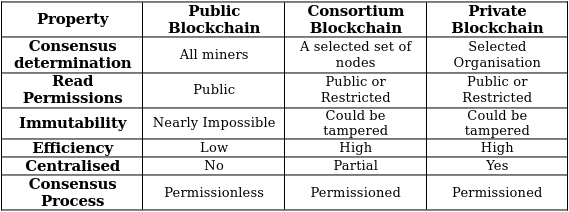
\includegraphics[width=0.7\textwidth]{assets/state-of-art/type-blockchains.png} % Change this to your image file
	\caption{State of art: blockchain types table}
	\label{fig:sample-image} 
\end{figure}

\begin{figure}[H]
	\centering
	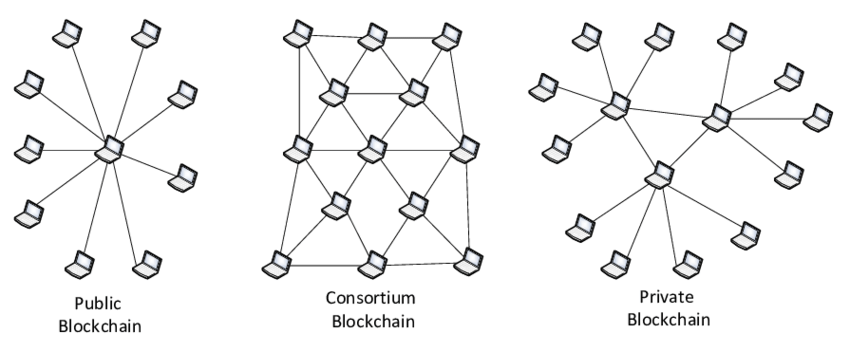
\includegraphics[width=0.7\textwidth]{assets/state-of-art/type-blockchains2.png} % Change this to your image file
	\caption{State of art: blockchain types visual representation,Source: \cite{private-vs-public-vs-consortium}}
	\label{fig:sample-image} 
\end{figure}

Each type of blockchain, irrespective of its classification, presents distinct advantages 
tailored to its particular use case. Public blockchains may be suitable for certain situations, 
while in others, it may be necessary to ensure private control through consortia or private blockchains.
The choice of which type of blockchain to implement ultimately depends on the specific service or application 
for which it is needed \cite{private-vs-public-vs-consortium}.

\subsection{Blockchain and Healthcare Sector}
The healthcare sector is a problem-oriented domain with intensive data usage and personnel
involvement, where the ability to access, edit, and trust data emerging from its activities 
is crucial for the sector's overall operations. Currently, healthcare institutions face a growing 
demand for data from the industry and research organisations. Simultaneously, unauthorised sharing, 
breaches and theft of sensitive data continually undermine public trust in these institutions, which 
can be fatal in certain critical level information's. A third issue involves bad and non standardized 
practises in the healthcare ecosystem, such as problems with medications, procedures, 
competencies and patient falsification. Given this set of challenges, it is necessary to 
explore alternative approaches to the existing ones. With key attributes such as decentralisation, 
distribution and data integrity, without needing third parties, blockchain technology can surge 
as a potential allie to fight this problems. In addition, this technology can also ensure and 
improve existing interoperability, information sharing, access control, provenance,immutability 
and analytics of data among stakeholders, along with an extensive set of features. This way, the 
healthcare sector is moving towards a new infrastructure capable of building and maintaining 
trust among all stakeholders speeding up innovation \cite{systematic-review-of-blockchain} \cite{healthcare-theft-data}.

The immutability offered by blockchain is a crucial option for health data, 
safeguarding health records and clinical outcomes and ensuring regulatory compliance when 
standardized practises get achieved. The use of smart contracts demonstrates how this 
technology can support business logic and ,by taking leverage of other technologies, 
potentially enhance processes of real-time monitoring of patients ,medical interventions, 
enhancing patient data security, reliability, privacy, availability and management 
of the infrastructure. It has the power to manage patient data, enabling the exchange of medical 
records between different healthcare institutions while maintaining a record and control over access 
to this data. Another application is related to the pharmaceutical supply chain and developing
measures against counterfeit drugs. Despite the substantial costs of developing new drugs,
including trials assessing the drug's safety and efficacy, smart contracts facilitate the 
informed consent procedure, improve identity management, and enhance data quality. Providing 
patients with access to manage their identity also allows the integration of the informed consent 
procedure, ensuring the privacy of individual health data \cite{blockchain-patient-control} 
\cite{blockchain-in-healthcare-2} \cite{blockchain-counterfeit}.

According to \textbf{IBM}, 70\% of healthcare leaders predict that the most significant 
impact of blockchain in the healthcare domain will be in improving the management of clinical 
trials, ensuring regulatory compliance, and establishing a decentralised framework for sharing
electronic health records \cite{IBM-reference}.

\subsubsection{Key Blockchain Benefits/Features When Applied to the Healthcare Sector}
Speaking about blockchain influence within the healthcare sector. To understand why 
this technology can be viable for biomedical and healthcare applications, the key 
benefits and advantages it presents to the sector are respectively data integrity, 
data traceability and data security due to the logic introduced in smart contracts
and it's cryptographic schema and the flexibility of supplying data, because the 
ledger is like a puzzle and when you share data the recipient can check if the data 
is actually valid using this puzzle. Furthermore, with the ongoing evolution of 
the healthcare landscape, blockchain technology plays an increasingly vital role, 
providing innovative solutions to tackle various 
challenges within the 
sector \cite{blockchain-distributed-ledger-biomedical} 
\cite{blockchain-research-challenges}.

\paragraph{A. Authentication} \mbox{}\\
Blockchain provides secure storage and ensures the authentication of records or other 
private information stored in blocks along the blockchain. This authentication process requires 
a specific private key linked to a public key to initiate the creation, modification, or viewing of 
information stored on the blockchain \cite{btc}.

\paragraph{B. Immutability} \mbox{}\\
This technology supports only creation and reading functions, 
making it challenging to alter data or records. As a result, blockchain is well-suited as an 
immutable ledger for recording critical information, including insurance claims records and confidential 
patient data. Immutability is established via a consensus mechanism whereby a network of nodes must collectively 
validate transactions before they are appended to the blockchain. Transactions are linked to each other which 
make a block and a block is also connected to the previous block, all cryptographically, thus creating a chain
of blocks that reinforces the security and integrity of the recorded data \cite{btc}.

\paragraph{C. Provenance} \mbox{}\\
The owner can only change ownership in the blockchain, following cryptographic protocols.
Furthermore, the origins of assets are traceable, allowing for verifying sources and data 
records. This traceability enhances the reuse of verified data. Therefore, the blockchain 
is well-suited for managing critical digital assets like patient consent records. This 
traceability is achieved through cryptographic techniques, ensuring a secure and 
auditable history of asset ownership changes.

\paragraph{D. Robustness/Availability}\mbox{}\\
Each node in the blockchain has a complete copy of the historical data 
record. This characteristic makes it well-suited for the preservation 
and continuous availability of important records, such as patients' electronic health 
records. Data distribution among nodes ensures redundancy, contributing to 
the blockchain's resilience and reliability for long-term data preservation. Combined 
with other existing technologies, this concept of Availability can be even more improved, 
making single nodes available even tought some failures occur \cite{btc}.

\paragraph{E. Security} \mbox{}\\
Blockchain technology can be a powerful allie of healthcare security, since it leverages advanced
encryption, distributed consensus and immutability if everything is well 
designed. Putting all features together, it may represent a strong resource when it comes to 
cyber threats, malicious actors within the organization and lack of integrity in the possessed data. 
To put it more clear, advanced encryption preserves data confidentiality, 
distributed consensus can prevent malicious actors from modifying the data if well designed 
and immutability, due to this encryption linkage that is usually assoated to a puzzle, can 
indeed make sure that the data is not tampered \cite{encryption-algorithms}.

\paragraph{F. Privacy} \mbox{}\\
Privacy comes along as another big pillar that, not only is important within the 
healthcare landscape, but also plays as a huge concern in every realm of information 
management. Blockchains usually come with a certain number of features that ensure privacy. 
In some types of blockchains the privacy is achieved by not knowing which person owns what (public), 
while in the other hand the privacy is achieved by \textbf{ACM's} (Access control mechanisms). Regarding 
the second way to achieve privacy,more concretely in the healthcare environment, this achievement is filled 
by facilitating secure sharing of medical information among authorized parties, enabling 
granular control over the access of healthcare data and by ensuring pseudonymity in transactions 
which by extension gives the blockchain usage benefits like authentication,immutability,provenance,
robustness,availability,security and privacy where all together improve security,transparency and privacy \cite{privacy-healthcare}.

\subsubsection{Implementation Requirements} 
To successfully implement a blockchain, a certain number of aspects must be fulfilled: interoperability, 
security, consistency, integrity, data immutability, cost and resource effectiveness, trust and transparency, 
and complexity \cite{blockchain-utilization-in-healthcare}.

These requirements are a must for establishing the groundwork for a resilient and efficient blockchain system
 tailored to healthcare needs which means that they are shared across multiple blockchain implementations. 
 The detailed examination of each requirement will provide insights into the necessary considerations for successful 
 implementation in the healthcare domain  \cite{implementation-requirements-blockchain}.

\paragraph{A. Interoperability} \mbox{}\\
Any organization and ,more specifically, healthcare systems encounter challenges ensuring interoperability, 
which represents a major barrier in health management systems. The lack of universal standards contributes to this issue. 
Altought standards are discussed every day,   blockchain technology can mitigate this issue by enabling the interoperability of 
electronic health systems with current healthcare systems.

This integration comes facilitated by blockchain due to the flexibility of most of the implementations(ex: \textbf{Hyperledger fabric}), 
where health information can be exchange across different systems, according to a before hand setting of rules, fostering a more 
interconnected and efficient healthcare ecosystem in a controlled and secure environment \cite{blockchain-utilization-in-healthcare}.

\paragraph{B. Data Security} \mbox{}\\
In cases where multiple entities are involved, there must be a way to ensure that data is secure. In order to ensure that this data 
is actually safe, there is the surging of Blockchain because it can ensure higher security, privacy, and trust among multiple parties 
compared to traditional healthcare systems. This is mainly because of the characteristics that were mentioned before. To mention the 
main reason for this to happen, increased privacy and trust by all entities is achieved by a consensus of nodes where the rules for 
establishing who can do what and what is determined as a valid transaction is also something that must be agreed between a consortium of 
organizations, where the number of organizations that must agree in these definitions depends also on the agreement of the involved. This 
creates transparency, is more easier to setup than by using a conventional technology because everything is just well and previous thought 
and enhances the overall security of patient data, instigating for a system where every action within the consortium or even outside is 
verifiable , traceable across the network and thereby valid \cite{blockchain-utilization-in-healthcare}.

\paragraph{C. Data Integrity} \mbox{}\\
Lack of data consistency of medical data is a major problem in the modern landscape. Data inconsistency can cause delays and higher 
costs in completing the overall health process for any patient, not speaking about research bad results since researchers that 
want to improve patient service rely on this data. Therefore, a blockchain-based healthcare system must ensure that health data 
is consistent and cannot be altered by unauthorised entities or malicious actors \cite{blockchain-utilization-in-healthcare}.

By correctly leveraging blockchain technology we can possibly guarantee data consistency, integrity and immutability by creating a 
tamper-resistant record of all transactions. This enhances health processes, providing a secure and unalterable history of each 
patient's medical data and even possibly setting rules to accept or dismiss information if the network provides something such 
as a smart contract, therefore providing integrity at the max level.

\paragraph{D. Cost and Resources} \mbox{}\\
Currently, healthcare systems are consuming more resources in terms of costs, computations, time, personnel and machinery. 
For example, in most transactions, the presence of intermediaries may lead to more delays or resources required to perform 
specific tasks. One of the key requirements when implementing a blockchain-based system is the possibility of reduction of costs and 
transaction delays that can be caused by third parties, multiple entities involved or any other reasons \cite{blockchain-utilization-in-healthcare}.

Blockchain technology increases processes effectiveness by eliminating intermediaries and possibly reducing the overall 
resource consumption, resulting in a more cost-effective and efficient healthcare system.
\paragraph{E. Trust and Transparency} \mbox{}\\
With the current healthcare system, it is necessary to build trust among various stakeholders to ensure more secure data 
storage and sharing processes. Maintaining complete trust and transparency becomes a significant challenge as data is stored 
and shared among multiple parties. A blockchain-based system eliminates the overhead of intermediaries and creates a deterministic 
source of data thus building more reliable and transparent healthcare systems.
By eliminating intermediaries, blockchain establishes a system where each transaction is verifiable, traceable, and transparent, 
building trust among stakeholders and preserving the integrity of health data.

This becomes all possible due to the cryptographic nature of blockchain, which creates less human interaction and 
by extension creates error prone processes and also removes probable bad actors that may be within those processes, which creates 
deterministic operations by extension.
\paragraph{F. Complexity} \mbox{}\\
Current healthcare systems involve multiple stakeholders and are more complex in storing, sharing, and processing medical data and other 
billing-related information. Therefore, one of the requirements for a blockchain healthcare system is to have fewer complex processes to 
prevent unnecessary complexities and delays at various stages of the process.
Simplifying processes within a blockchain-based healthcare system streamlines the overall workflow, reducing complexities and enhancing
efficiency. This ensures smoother stakeholder interactions and minimises delays in critical stages of healthcare processes.

Altought the processes can become simpler, there must be a conscious thought from the organization that depending of the design of 
the blockchain solution the system may become complex. Standardized approaches, operational guides and recovery plans usually 
are ways to also remove this complexity more into the nature of managing the network.

\subsubsection{Implementation Challenges/Issues} 
Issues and challenges must be considered when contemplating the implementation of a blockchain-based health system. The challenges 
identified in the research are listed and detailed throughout this section \cite{blockchain-utilization-in-healthcare}.

\paragraph{A. Security and Privacy} \mbox{}\\
Looking to the security aspect, there is a concern about ACM's (Access control mechanisms like for example ACL's),authentication 
and non-repudiation which can be a extreme barrier when it comes to offer overall data integrity,confidentiality and availability of 
this sensitive information. Restricted access to controls, querying ,writing and provide a correct logic to handle information are 
the main mechanisms to making sure we achieve the wanted result, which can be challenging since there other problems associated with 
this. As a example, non-standardized encryption protocols create heterogeneous processes between organizations and even within the same 
organization, imposing a challenge when it comes to access information \cite{med-rec}.

\paragraph{B. Interoperability} \mbox{}\\
Interoperability is a crucial requirement for the healthcare sector since the proper organization or multiple organizations 
needs to access this data, either for own usage,investigation,giving information to a supplier or any other entity that requires 
the usage of a given slice of data. This involves sharing and transferring data between different sources, which is not optimal. The 
biggest issue with interoperability is , in the current methodology, that data storage is done in different sources within the healthcare 
institution. This is due to the fact of how Centralized data storage operates and it poses a problem for healthcare providers as it 
consolidates all health records in a single point but with multiple data sources. This becomes a issue arising from fragmentation of 
health data, slow access, and the quality and quantity of data for medical research \cite{blockchain-interop}.

Many records are generated daily and stored centrally in different hospitals. Since the data is stored across various hospitals 
this may result in the loss of data and the patient needs access to the contained data. Blockchain technology can come into play to 
ensure interoperability among all hospital systems, since it helps sharing data in a secure and effective way. With its decentralised,
distributed ledger and the possibility to implement various rules and business logic in the processes, blockchain faces the challenges of 
centralised data storage because it allows more efficient and secure health data exchange between 
different healthcare entities, ensuring data integrity and accessibility \cite{med-rec}. 

\paragraph{C. Data Sharing} \mbox{}\\
Data sharing is a huge problem when considering healthcare records. Sharing these can be challenging, as unfortunately the 
records of an individual may be stored in various locations. In order to a Patience have a comprehensive view of it's state, 
behind the hoods, it must gather records dispersed across multiple healthcare units which sometimes is not feasible and,also 
unfortunately, this also applies to healthcare providers as they need access to up-to-date patient data if records are located 
elsewhere. Since this records are dispersed in a vast number of institutions, this becomes a challenge for seamless sharing, due 
to bureaucracy and because it's hard to gather information from a vast number of points. 

Now, this becomes even worse if some data is not meanted to be shared to certain entities. As instance, hospitals and 
insurance payers may be reluctant to share data too easily with other entities. One reason could be that the hospital 
wants to keep the prices at which it gets the products for it's activity. Thus, mechanisms must be created in order to tell what 
which entity can access from where. Blockchain offers this if well implemented, creating a enhance data sharing in healthcare by 
establishing a secure and transparent mechanism. It enables a decentralised approach to data storage and sharing, ensuring that 
stakeholders have controlled access to relevant and up-to-date information while maintaining data integrity \cite{med-rec}.

\paragraph{D. Mobility} \mbox{}\\
Since there is a substantial rise in smart devices,sensors and other kind of technologies, mobility is a important characteristic 
that the data must have. This becomes very hard since by moving data we must make sure that it remains secure and that it complies 
with legal requirements. With this in mind, blockchain is a suitable solution to have this moving of data respecting the business logic, 
empowering users with real time access to their medical records, ensuring the best security standards \cite{chainmob}. 

\paragraph{E. Transparency and Confidentiality} \mbox{}\\
The transparency of information during a transaction is also very important, altought often seen as a drawback. In a blockchain, 
everyone can see everything, resulting in higher transparency but lower confidentiality. Even  despite using hash values for 
anonymity, users can still potentially be identified by analysing transaction publicly available transaction information. 
This poses a threat particularly for critical healthcare applications where patient-related data is sensitive and 
confidential \cite{confidentiality-and-transparency}.

\paragraph{F. Speed and Scalability} \mbox{}\\
A real issue is real-time healthcare applications based on blockchain. This is because transaction times can vary 
depending on the protocol used, number of nodes within the consensus, network, current volume of transactions and 
other constraints. In other words, there must be careful thinking in terms of what it is needed and the amount of 
decentralization that we want so it does not affect the available computing capabilities and the volume of medical 
transactions required for such healthcare systems. Also, by recurring to horizontal scaling there may be a possibility 
of increasing the number of components that serve requests without actually increasing the number of members of the consensus, 
which could be valuable in certain situations but further benchmarking is required to see until each measure it 
can help \cite{ethereum-scaling}.

\paragraph{G. High Development Costs} \mbox{}\\
Healthcare systems based on blockchain can incur high development and operation costs. Altought the solution excels in 
flexibility, refactor the way the things is currently done takes resources. With this in mind, understanding how can it 
be done at the minimum usage of resources is something that is seem as challenge but there must be careful thinking on this 
matter \cite{hyperledger-cost}.

\paragraph{Standardisation} \mbox{}\\
Because there are a lot of uncertainties along the way, it's always important to seek standardization. This is very 
important, since standards usually occur from given situations that were faced before and it becomes precedent to 
actually use already well established best practises that faced the same exact problem, precisely because they were 
proven to solve the given problem. With this in mind and ,specially concerning the healthcare, there must be specially 
defined what types of data, size , format and other kind of characteristics can be recorded into the blockchain. Also, there 
must exist clear guidelines about  which data should be stored on-chain or off-chain. Having on hands these kind of information is 
more than greater to ensure integration between blockchain technology and the healthcare systems \cite{blockchain-standards}.

\paragraph{Cultural Resistance} \mbox{}\\
Stakeholders that were used to other ways of managing data may present resistance to change. Is it either by relying on 
paper-based procedures and Electronic Health Records or other online services. This personal is even more skeptical to actually 
have a platform that makes sharing of data something common, which can be revealed as being a hell of a challenge, also because 
there was also times were a hybrid paper-based and online services were actually useful, because there were cases where the online 
services stopped working and because they had the paper from older stakeholders, they were able to function almost at 100\%. Besides 
reveiling all of the benefits we also must present blockchain as something that hardly could become unavailable and availability 
itself is something as much harder as changing people's minds. To put it clear, it is important to gain broadly acceptance of this 
new way of doing things but also deserve the trust from the stakeholders \cite{cultural-resistance}.

\subsubsection{Applications of Blockchain Technology in the Healthcare Sector}
Since this technology is emergent, it has been still gathering interest by the researchers, but fortunately more and more 
research use cases are surging and this may result in further future solutions that can benefit the healthcare landscape. The most 
discussed applications of blockchain in this precise space is for information exchange,transactions between patients,transactions 
between providers,transactions between payers and transactions between a whole other number of relevant parties. The potential of this 
is huge and there is plenty of expectations regarding the further usage of this concept.
With this on scope, and because there is some research about this matters, there is mentions to the exact current known applications 
more ahead.

\paragraph{A. Electronic Medical Records} \mbox{}\\
A current usage of the blockchain technology is for management of eletronic medical records (or EMRs), often also called personal 
health records (PHRs). These records are usually meanted for creation,storage and management of the patient data. Blockchain, if 
implemented, can take a huge responsibility in the management of this data, determining exactly how it is shared, how it is processed
and how it is used. Now, because of the nature of the immutability of this technology, the risk of tampering becomes almost zero because 
once some information is recorded neither the doctors or the patients can alter this data. Also, because of cryptography and business logic, 
data will for sure only be recorded if it is actually valid thus enhancing the integrity of the data in question not speaking about this 
could actually influence the security and privacy of the data since the data can only be decrypted by using the patient private key for 
example, but this depends of the cryptographic scheme that is in place. Key attributes such as decentralization, immutability, data provenance, 
reliability, robustness, smart contracts, security, and privacy make blockchain an ideal solution for storing and managing EMRs. As an
example, there is a application of this in MedRec, a decentralized record management system developed by Azaria, Ekblaw, Vieira, and 
Lippman. This solution enables patients to access their medical information in real time across different healthcare services and treatment 
locations. It gives the power to patients to securely share their records and decide who the access of it is guaranteed. Besides this and ,
because of the modular design that integrates existing local data storage systems, there is interoperability for both doctors and 
patients \cite{apps-block-healthcare}.

\paragraph{B. Clinical Data Sharing} \mbox{}\\
Clinical data sharing is another crucial application of blockchain in the healthcare sector. It enables secure data exchange 
facilitating data sharing among various entities in the system. Confidential and crucial patient information is stored within 
electronic health records (EHRs) and electronic medical records (EMRs), highlighting the need for secure storage, processing and 
access. Sharing this data among healthcare stakeholders is essential for improving service quality, but it also requires robust 
transparency and accountability measures.
By leveraging blockchain these challenges are gone, because there is a record of all this transactions in a distributed ledger 
creating security and transparent data sharing. All participants can view the transactions, which creates a friendly environment 
for managing clinical data in a secure way.

An example of this is applied to clinical data sharing is HealthVerity. This solution leverages blockchain to enable secure and transparent 
clinical data exchange of data between healthcare organizations,payers and research organizations which promotes further collaboration in 
research and clinical analysis. With this, the organizations can deal easily with data access, interoperability and privacy. By creating 
this environment, this project supports research,analysis and data-driven innovation within the healthcare sector which influences 
several future work that enhances the healthcare services \cite{block-apps-increased-transparency} \cite{health-verity}.

\paragraph{C. Global Data Sharing} \mbox{}\\
The most frequently spoken subject while speaking about blockchain is data sharing, but a even more extensive 
subject is when we apply this at the global context. If applying this concepts regionally is hard, imagine trying to expand 
this standardized solution to multiple organizations across the globe, the potentiality is immense but so it is the complexity 
of such systems. Imagine if a patient wants to be treated in a foreign healthcare provider, this means lots of bureaucracy just 
for this institution to have access to this patient data which takes time that sometimes lacks. By recurring to blockchain, all 
of this bureaucracy can still be done but quickly as fast as the procedures in a chaincode can be, depending of the implementation 
in use of course, and still give patients the control to decide who can access it's data, which is a requirement to ensure safe and 
effective treatment abroad. In simple terms, this technology can deliver optimal care regardless of the location.

An example of this is Health Wizz, a platform focused on healthcare and it leverages blockchain for supplying secure and transparent 
solutions for storing and sharing healthcare data across the globe. Users have the opportunity to store and manage their health data, which 
includes medical history, test results, prescribed medications and other resources. Health Wizz creates immutable and tamper-proof records,
ensures reliability and authenticity of information, data integrity, privacy and secure sharing between participants \cite{health-wizz} 
\cite{blockchain-pharmaceutical-cold-chain}. 

\paragraph{D. Medical History Maintenance} \mbox{}\\
Having a medical history is something particularly interesting and important, because it keeps track 
of patient records which gives insights about, for example, when a patient visits multiple hospitals and there is a need to avoid 
redundant analysis over the patient like for example doing the same analysis multiple times. If this history is well maintained and 
shared across institutions, then there will be the reduction of redundant processes when treating the patient, reducing costs,risks and
time needed for the observation.

Blockchain offers a reliable way to maintain and store this history and , at the same time, offers more power to the patient which chooses or 
not to share its personal information. This increases privacy and consent management. In other words, it offers a extra layer of trust 
preserving the integrity of medical records over time, preventing as well tampering and unauthorized alterations.
Medicalchain, a technology company, leverages all of this to offer accurate data record with meticulous updating of the data and its 
history. This is very valuable if a patient goes to multiple healthcare institutions \cite{medicalchain}.

\paragraph{E. Health Data Access Control} \mbox{}\\
The more data retained, the more difficult it is to secure it and because of this there is a need to create mechanisms to make users 
aware of who accessed their data, because by only giving them power to decide who sees it makes the user unaware of those that can be inside 
of a given group and their access can be camouflaged making the user more vulnerable than ever. Therefore there is a 
need of giving this power to users: allow or not allow some entity to access its data, check who is seeing its data, check who is storing 
its data and check who is sharing its data. Blockchain helps by giving potentially all of this to the user, simply by leveraging smart 
contract to enforce rules and permissions.

An example of this application is Coral Health, which uses blockchain to make easier the secure sharing and access to patient information. 
Patients can trust that their medical records remain the same and the platform also connects them to other participants in the healthcare 
service such as doctors,scientists,lab technicians and public health authorities. Using the blockchain is a huge life savior in this 
situation because besides of the benefits that were mentioned earlier, there is also administrative automated processes and deterministic 
operations that are error prone for accurate data and treatments for the given patients \cite{coral-health}.

\paragraph{F. Billing/Payments} \mbox{}\\
Payment system may be complex and prone to fraud, leading to requiring more resources and time than needed. To face this problem 
there are usages of blockchain to simply and speed up the payment process when comparing with traditional payment methods. Using blockchain, 
invoice processing and payment processes flow faster and this removes barriers from the activities, there is no need for intermediaries, 
prevents fraud, helps stakeholders access the data and makes the data more secure,private and less prone to cyberattacks. 

Blockchain has a powerful tool called smart contracts - Self-executing agreements with terms encoded directly into the system. Doted of 
this, the automation of processes is possible because smart contracts provide all the business logic needed to come up with what is needed 
in that flow and by extension it also reduces administrative burden, minimizes errors and disputes, contributes to more efficiency, gives 
more transparency in the payment ecosystem, provides security and fraud-prone payments.

As an example there is the project PokitDok, a platform which uses blockchain to facilitate payments and transactions in healthcare. 
Within this project DokChain was developed, a private blockchain that references off-chain file systems that, by incorporating smart 
contracts retrieves data from health insurers and payers in real time, enabling real-time decisions on insurance claims. After a patient 
treatment, all of the information about the treatment is available to all stakeholders and thereby there is a calculation of the given costs 
by leveraging smart contracts. Also, the platform makes calls to API's to assess a patient's payment risk, enabling patients to schedule 
and pay for healthcare services, automating payments and verifying benefits instantly \cite{poki-dok}.

\paragraph{G. Biomedical Research and Education} \mbox{}\\
When it comes to do research or even gather information that make people conscious of a given reality for the sake of education there 
are problems that must be faced. Especially in healthcare, there are questions regarding the acceptance of the participants for them to 
land their data. Also, in cases where the sources of data are not that valid, data can give bias to those that analyse it, which 
unfortunately is good for a certain number of malicious actors that just want to make sure that their point is correct where in 
reality it isn't. To go against this problems, not considering the analysis of the source and doubting the author in question and 
it's purpose, there is the possibility of using blockchain which can serve as a powerful allie against falsification,reducing the omission 
of unfavorable clinical research outcomes and maintainability of data integrity. Also, by using historical data which the blockchain 
maintains, there is the possibility of questioning current surprising results, giving us the possibility to question what caused such 
variability in them, thereby aggregating hints about the possible bad introduction of those inputs. 

An immutable record of patient consent enables regulators to monitor trial patterns and ensure compliance with informed consent 
regulations. With this, there is also the possibility to detect fraudulent form consents, which are a form of clinical fraud, resulted 
from record tampering and fabricated patient consent. If implemented well, blockchain can make sure that only patient permitted 
participants, can access or use in multiple their data. Thereby, for this concrete situation, there must be mechanisms to consent,revoke 
consent,see which entities are taking advantage of the consent and this must be per item that the user retains. This not only gives power 
to the patients, but it removes a lot of bureaucracy in releasing their data for better purposes like research and it also helps for 
auditing clinical teams,researchers and regulatory authorities.

As an example, there is this project called Shivom Project, which aims to implement blockchain in genomic data technologies. With this in 
mind, users of this platform can store, share and monetize their genetic information. By leveraging this large genomic datasets, the project 
aims to make research and treatment discovery easier, while participants maintain control over who uses its data or not \cite{crunchbase}. 

\paragraph{H. Pharmaceutical Supply Chain} \mbox{}\\
When it comes to the supply chain, there are a lot of mentions to blockchain but in a particularly more focused in 
healthcare perspective, there is the case of the pharmaceutical industry. This is because, unfortunately there are cases of counterfeit 
or substandard drugs that can cause harmful issues to patients.

By using blockchain, every transaction that involves probably risky products is recorded from the production,distribution 
and the delivery to the end consumer. This occurs because, in case of malicious intent within this chain, there are records that 
give hints about where the product came from, thereby actions can be taken in order to solve this kind of issues. With this in mind, 
there is a barrier against drug alterations and modifications within the chain, counterfeit drugs and stealing. With this, poor quality 
drugs are easily tracked until their source, helping healthcare institutions to meet safety and regulatory standards in pharmaceutical 
supply chains.

As an example, \textbf{IBM} launched projects with pharmaceutical manufactures,distributors and hospitals to demonstrate the feasibility 
of blockchain-based solutions \cite{blockchain-implementation-review-conceptual}. 

\paragraph{I. Equipment tracking}  \mbox{}\\
Equipment tracking is closely related to supply chain, the difference is that this concerns the life after the delivery process and 
it concerns who retains what within the organization or what does the stakeholders retained before. Because of the immutable nature of 
the history inside of blockchain records, blockchain stands as an huge countermeasure against theft,loss,movement and reordering of medical 
devices. By preventing alteration and deletion of the location history, there are plenty of dollars that are saved, making this solution a 
tamper-proof against this unfortunate situation.

Additionally, in case the usage of this technology is guaranteed, there are less costs associated with personal and less errors occur due 
to their deterministic nature making the life easier for those that require this equipment's for their work like nursers,porters and staff 
support.
As an example, Chronicled exists as a project that focuses on supply chain solutions but that also offers solutions around product tracking. 
What makes this product more interesting is that product tracking works as an extension of supply chain tracking which goes in accordance to 
the closely related relationship that was mentioned before. Putting in another words, this product leverages blockchain to not only track 
products in its supply chain but also to track the products after the delivery, which creates immutable,transparent and valid records that 
provide reliable audit trail for each product \cite{chronicled}.

\paragraph{J. Health Data Analysis} \mbox{}\\
Data has become something that is more valuable than gold, because it can help us understand the best way to operate in various realms 
of the human devour. It spots behaviors, characteristics about something that no one spotted and helps businesses to meet optimal solutions 
for difficult problems. In order to achieve this, not speaking only about data itself, analysis must be done and, in order to make good 
analysis, data must be also of fine quality in terms of integrity, verificability and ownability. 
If done correctly, data analysis can revolutionize the healthcare field in such a way that patterns can get identified, medicine can be 
tailored to patience characteristics and preventive measure can be taken. 

Blockchain can take an huge responsibility in terms of making this possible, because it safeguards the integrity and privacy of the data, 
addressing also concerns around security and confidentiality which can lead healthcare institutions to significant breakthroughs in medical 
research and patient care becomes better.
As an example, Nebula Genomics, makes analysis of genomic data that comes from a blockchain and , in this precise way, reshapes the 
genomic data market. It creates a market where buyers, such as sequencing facilities, drug design companies and health organizations,
can access genomic data. Individuals use this platform to discover their genetic variants,disease predispositions and get compensated by 
allowing third parties to access their data, while still maintaining privacy \cite{potential-blockchain-tech}.